\documentclass{article}

\title{Square joy: trapped rainwater}
\subtitle{Solving the trapped rainwater problem in J.}
\reddit{https://www.reddit.com/r/apljk/comments/ssyl00/blog_post_square_joy_trapped_rainwater/}
\date{2022-02-15}
\modified{2024-03-03}

\keyword{j}
\keyword{arrays}
\keyword{puzzles}

\begin{document}
\section*
In this article, we'll explore one of my favorite programming puzzles using the \href{https://en.wikipedia.org/wiki/Array_programming}{array programming} paradigm.

\section{the-why}{But why?}

I am always looking for new perspectives on software engineering and programming.
My views on computing changed profoundly when I discovered the array programming paradigm a few years ago.

For me, the hardest and the most rewarding part of array programming is coming up with simple idiomatic solutions.
Idiomatic solutions require knowledge of many little tricks array-wrangling wizards developed in their chambers over the last fifty years.
I would love to learn or rediscover these tricks, and I hope you might derive some pleasure and insights from reading about my little discoveries.

In this article, we'll use the \href{https://www.jsoftware.com/#/}{\sc{j} programming language}.
Why \sc{j} and not, say, \href{https://dyalog.com/}{\sc{apl}}?
\sc{j} is easier to type on most keyboards, and it's \href{https://github.com/jsoftware/jsource}{open source}.

The code in this article will look like line noise if you aren't familiar with \sc{j}.
Don't be discouraged; this reaction is typical when working with \sc{j}.
I'll explain most of the steps, but the steps might still look like black magic sometimes.
My goal is not to explain every aspect of the language but to demonstrate the problem-solving approach.

Time to have some fun!

\section{the-problem}{The problem: heavy rains in Flatland}

Imagine living in a two-dimensional city where all buildings have the same unit width and stand next to one another.
We don't like rain very much: the two-dimensional water gets stuck between the buildings forever, forming pools.
As city architects, we know the heights in units of all the buildings.
We need to compute how much water (in square units) accumulates between the buildings after heavy rain.

More dryly: given an array of non-negative integers \em{H}, representing heights of unit-width bars placed next to one another, compute the total area of water trapped by the configuration after a rain.

\subsection{example-2d}{Example}
\begin{tabular*}{r l}
    \em{Input} & \code{0 1 0 2 1 0 1 3 2 1 2 1} \\
    \em{Output} & \code{6} \\
\end{tabular*}

\newline

\begin{figure}
  \marginnote{mn-example}{The configuration of bars with heights 0, 1, 0, 2, 1, 0, 1, 3, 2, 1, 2, 1, and the water trapped by this configuration.}
  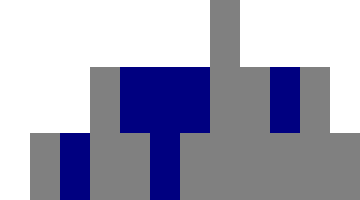
\includegraphics{/images/04-viewmat-2d.png}
\end{figure}

\section{a-solution}{A solution}

A natural first question is: what is the water level above each bar?
If we knew that, summing contributions of levels above each bar would give us the answer.

So, let's focus on the bar at an arbitrary index \math{i}.
What would stop the water from flowing out?
Another bar that is higher than \math{H\[i\]}.
Furthermore, we need bars higher than \math{H\[i\]} on \em{both} sides of \math{i} for the water to stay.
So, the water level at index \math{i} is determined by the minimum of the highest bars on the left and right.

Computing the highest bar to the left and to the right for each index is not efficient: we would need to make \math{O(N\sup{2})} steps.
Luckily, we can eliminate a lot of duplication in this computation.
Instead of running the search from each position in the array, we can precompute the left and right maxima for all positions in two sweeps.

The algorithm to compute the running left maximum is called \href{https://en.wikipedia.org/wiki/Prefix_sum}{prefix scan}.
We can compute the right maximum by running the same scan from right to left (i.e., performing a suffix scan).
Taking the minimum of precomputed left and right maxima gives us the water level at each point.
The difference between the water level and the bar height gives us the volume of water trapped at this position.
Summing up all volumes gives us the answer.

\section{translating-to-j}{Translating our idea to J}

\sc{j} is an interpreted language and it has a \href{https://en.wikipedia.org/wiki/Read%E2%80%93eval%E2%80%93print_loop}{\sc{repl}}.
It's pretty standard for \sc{j} programmers to build solutions incrementally by trying snippets of code in the \sc{repl} and observing the effects.
The code in this article is also an interactive \sc{repl} session that you can replicate locally.
Let us get some data to play with.

\begin{code}[j]
    NB. Comments start with the symbol NB.
    NB. I use PascalCase for data (“nouns”)
    NB. and snake_case for functions (“verbs”).

    NB. User input is indented.
NB. Machine output is not.

    H =. 0 1 0 2 1 0 1 3 2 1 2 1
\end{code}

The next item on our agenda is computing the left and right running maxima.

\begin{verbatim}[j]
    >./\ H
0 1 1 2 2 2 2 3 3 3 3 3

    >./\. H
3 3 3 3 3 3 3 3 2 2 2 1
\end{verbatim}

Wait, where is all the code?
Let me break it down.
In \sc{j}, \href{https://code.jsoftware.com/wiki/Vocabulary/gtdot#dyadic}{\code{>.} (max)} is a verb (\sc{j} word for "function") that, when you use it dyadically (\sc{J} word for ``with two arguments''), computes the maximum of the arguments.
It's easy to guess that \href{https://code.jsoftware.com/wiki/Vocabulary/ltdot#dyadic}{\code{<.} (min)} is an analogous verb that computes the minimum.

The single character \href{https://code.jsoftware.com/wiki/Vocabulary/slash}{\code{/} (insert)} is an adverb (\sc{j} word for ``function modifier'') that takes a dyadic verb to the left and turns it into a verb that folds an entire array.
Why is it called ``insert''?
Because it inserts the verb between elements of the array it operates on.
For example, summing up an array is just \code{+/}.

\begin{verbatim}[j]
    NB. +/ 1 2 3 4    <->    1 + 2 + 3 + 4

    +/ 1 2 3 4
10
\end{verbatim}

But wait, we want running results, not just the final maximum.
That is a job for adverbs \href{https://code.jsoftware.com/wiki/Vocabulary/bslash}{\code{\\} (prefix)} and \href{https://code.jsoftware.com/wiki/Vocabulary/bslashdot}{\code{\\.} (suffix)}.
These take a verb and produce a new verb that applies the original verb to all prefixes/suffixes of an array, forming a new array.

\begin{verbatim}[j]
    NB. +/\  1 2 3 4    <->    (1) (+/ 1 2) (+/ 1 2 3) (+/ 1 2 3 4)
    NB. +/\. 1 2 3 4    <->    (+/ 1 2 3 4) (+/ 2 3 4) (+/ 3 4) (4)

    +/\ 1 2 3 4
1 3 6 10

    +/\. 1 2 3 4
10 9 7 4
\end{verbatim}

We already know enough to compute water levels for our example:

\begin{verbatim}[j]
    (>./\ H) <. (>./\. H)
0 1 1 2 2 2 2 3 2 2 2 1
\end{verbatim}

We need to subtract the bar heights and sum up the results.
We can get away with tools that we already know:

\begin{verbatim}[j]
    NB. Look at the picture in the example and convince yourself that the
    NB. water amounts we computed are correct.

    ((>./\ H) <. (>./\. H)) - H
0 0 1 0 1 2 1 0 0 1 0 0

    +/ ((>./\ H) <. (>./\. H)) - H
6
\end{verbatim}

This solution is remarkably concise.
Believe it or not, we can make it even shorter.
Look at the argument we repeated three times and at all these parentheses!
If only we could move some of those out\ldots

\begin{verbatim}[j]
    +/@((>./\ <. >./\.) - ]) H
6
\end{verbatim}

Such terse expressions that combine functions without mentioning their arguments are called \href{https://www.jsoftware.com/help/jforc/tacit_programs.htm}{tacit}.
I won't explain how to form these expressions here, but I encourage you to learn more about tacit programming independently.

Let us bind our beautiful tacit expression to a name.

\begin{verbatim}[j]
    trapped =. +/@((>./\ <. >./\.)-])
    trapped 0 1 0 2 1 0 1 3 2 1 2 1
6
\end{verbatim}

The full implementation of our idea now fits into 12 \sc{ascii} characters.
One surprising property of array languages is that it's often not worth naming functions.
Their entire body is shorter and more expressive than any name we could come up with.

\section{drawing-solutions}{Drawing solutions}

Knowing the answer is excellent, but being able to \em{see} it at a glance would be even better.
In this section, we'll write code to represent solutions visually.

What would we like to see in that picture?
We want to tell the space from the buildings and water pools.

Let us start by drawing the original problem first.
We know how to compute maxima: \code{>./ H}.
Now we need to build a matrix \math{max(H)} rows by \math{length(H)} columns.
The idiomatic way of doing this is using our old friend \href{https://code.jsoftware.com/wiki/Vocabulary/slash#dyadic}{\code{/} (table)} in a new disguise. 
When used as \code{noun1 verb/ noun1}, slash builds a \math{length(noun1)} by \math{length(noun2)} table, where each cell \math{i, j} is filled with the value computed as \math{noun1\[i\] verb noun2\[j\]}.

Let's make a multiplication table to understand how it works.
We'll also need \href{https://code.jsoftware.com/wiki/Vocabulary/idot}{\code{i.} (integers)}, the function that takes an integer and makes an arithmetic progression of the specified length starting at zero.

\begin{code}[j]
    i. 10
0 1 2 3 4 5 6 7 8 9

    NB. When the input is negative, the progression is descending.
    i. _10
9 8 7 6 5 4 3 2 1 0

    (i. 10) */ (i. 10)
0 0  0  0  0  0  0  0  0  0
0 1  2  3  4  5  6  7  8  9
0 2  4  6  8 10 12 14 16 18
0 3  6  9 12 15 18 21 24 27
0 4  8 12 16 20 24 28 32 36
0 5 10 15 20 25 30 35 40 45
0 6 12 18 24 30 36 42 48 54
0 7 14 21 28 35 42 49 56 63
0 8 16 24 32 40 48 56 64 72
0 9 18 27 36 45 54 63 72 81
\end{code}

Note that there is no particular boolean type in array languages.
They use integers instead: false is zero, and true is one.

\begin{code}[j]
    NB. Here, we build a table using the verb “less” (<).
    (i. 5) </ (i. 5)
0 1 1 1 1
0 0 1 1 1
0 0 0 1 1
0 0 0 0 1
0 0 0 0 0
\end{code}

We have all the tools we need to display our problems and solutions.

\begin{code}[j]
    NB. Compute the maximum of H.
    >./ H
3

    NB. Negate the maximum of H.
    - >./ H
_3

    NB. Make a descending progression that has the length of H maximum.
    i. - >./ H
2 1 0

    NB. Make a “less” table from the progression above and H.
    (i. - >./ H) </ H
0 0 0 0 0 0 0 1 0 0 0 0
0 0 0 1 0 0 0 1 1 0 1 0
0 1 0 1 1 0 1 1 1 1 1 1
\end{code}

If you squint a bit, you will see in the pattern of zeros and ones above the configuration of bars corresponding to \math{H}.
We already know how to compute water levels.
Let's add them (quite literally) to the picture.

\begin{verbatim}[j]
    NB. Make a similar “less” table, but use water levels instead of just H.
    (i. - >./ H) </ ((>./\ <. >./\.) H)
0 0 0 0 0 0 0 1 0 0 0 0
0 0 0 1 1 1 1 1 1 1 1 0
0 1 1 1 1 1 1 1 1 1 1 1

    NB. Add two “less” tables component-wise.
    ((i. - >./ H) </ ((>./\ <. >./\.) H)) + (i. - >./ H) </ H
0 0 0 0 0 0 0 2 0 0 0 0
0 0 0 2 1 1 1 2 2 1 2 0
0 2 1 2 2 1 2 2 2 2 2 2
\end{verbatim}

Look carefully at the matrix that we got.
Zeros correspond to empty spaces, ones---to water pools, twos---to bars.

Let's extract and name the verb that converts an instance of our problem into a matrix with classified cells.
Again, I won't explain how this tacit expression works, but I am sure you can see a lot of common parts with the expression above.

\begin{verbatim}[j]
    pic =. ((i.@-@:(>./) </ (>./\ <. >./\.)) + (i.@-@:(>./) </ ]))
    pic H
0 0 0 0 0 0 0 2 0 0 0 0
0 0 0 2 1 1 1 2 2 1 2 0
0 2 1 2 2 1 2 2 2 2 2 2
\end{verbatim}

We are one step away from turning this matrix into a picture.

\begin{verbatim}[j]
    (pic H) { ucp ' ░█'
       █    
   █░░░██░█ 
 █░██░██████
\end{verbatim}

\code{ucp} is a built-in verb that constructs an array of Unicode codepoints from a \sc{utf}-8 encoded string.
\href{https://code.jsoftware.com/wiki/Vocabulary/curlylf#dyadic}{\code{\{} (from)} is at the heart of our drawing trick.
This verb selects items from the right argument according to the indices from the left argument.
The effect is that all zeros got replaced with a space, ones---with a watery-looking glyph, and twos---with a solid rectangle.

Our pseudo-graphics look quite impressive already, but we can do even better.
\sc{j} comes with a convenient \href{https://code.jsoftware.com/wiki/Studio/Viewmat}{viewmat} library that can visualize arrays.

\begin{code}[j]
    require 'viewmat'
    viewmat pic H
\end{code}

\begin{figure}
   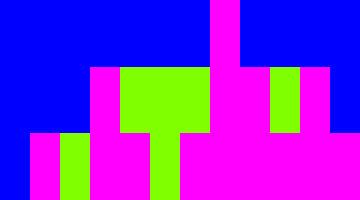
\includegraphics{/images/04-viewmat-2d-raw.png}
\end{figure}

That image looks quite good, but the colors are too psychedelic.
Let's use a more neutral color scheme.

\begin{code}[j]
    (255 255 255 , 0 0 128 ,: 128 128 128) viewmat pic H
\end{code}

\begin{figure}
   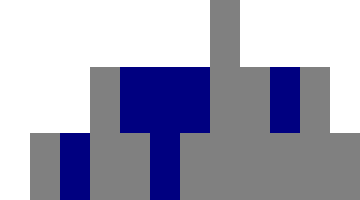
\includegraphics{/images/04-viewmat-2d.png}
\end{figure}

Ah, much better!
Now you know how I got the picture for the example.

Alternatively, we can use the \href{https://code.jsoftware.com/wiki/Plot}{plot} package and draw our solution as a stacked bar chart.
However, this approach needs more configuration and is slightly more cumbersome than \code{viewmat}.

\begin{verbatim}[j]
    require 'plot'
    'sbar;color gray,blue;aspect 0.5;barwidth 1;edgesize 0;frame 0;labels 0 1' plot H ,:  ((>./\ <. >./\.)-]) H
\end{verbatim}
\begin{figure}
    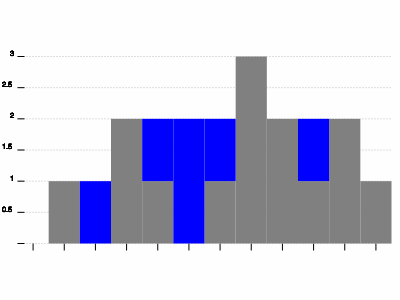
\includegraphics{/images/04-plot-2d.png}
\end{figure}

\section{3d}{Breaking out of Flatland}

\epigraph{One must always generalize.}{Karl Jacobi}

One of the ways to better understand a problem is to generalize it.
Let's break out into the third dimension.

Given a \em{two-dimensional} array of non-negative integers \math{H}, representing heights of square-unit bars placed next to one another, compute the total \em{volume} of water trapped by the configuration after it rains.

To make the problem more concrete, let's inspect a few instances.
We'll use \href{https://code.jsoftware.com/wiki/Vocabulary/tilde}{\code{~} (reflex)} adverb to save us some typing.
This adverb takes a verb and produces another verb that duplicates its right argument and passes the copies as the left and the right argument of the original verb.

\begin{code}[j]
    NB. +/~ X   <->   X +/ X
    NB. A cone that traps no water.
    +/~  (i. 4) , (i._4)
0 1 2 3 3 2 1 0
1 2 3 4 4 3 2 1
2 3 4 5 5 4 3 2
3 4 5 6 6 5 4 3
3 4 5 6 6 5 4 3
2 3 4 5 5 4 3 2
1 2 3 4 4 3 2 1
0 1 2 3 3 2 1 0

    NB. An inversed cone that traps water in the middle.
    +/~  (i. _4), (i. 4)
6 5 4 3 3 4 5 6
5 4 3 2 2 3 4 5
4 3 2 1 1 2 3 4
3 2 1 0 0 1 2 3
3 2 1 0 0 1 2 3
4 3 2 1 1 2 3 4
5 4 3 2 2 3 4 5
6 5 4 3 3 4 5 6
\end{code}

\subsection{solution-3d}{Solution}

Let's play the same trick: pick an arbitrary place on the grid and think of the water level we'll observe at that place.
This time, the problem is a bit trickier because there are many more ways for the water to flow.
We must consider all possible paths through the grid.
For each path, there is the highest bar that the water will have to flow through.
The water will choose a path where that highest bar is the lowest among all paths.
The height of that bar will determine the water level at that position.

Running a graph search from each point is very inefficient.
Luckily, we do not have to.
All our searches have the same destination, the ``ground'' outside of the grid!
We can invert the problem and ask: what is the most efficient way for the water to ``climb up'' the bars?
In this formulation, a single run of a shortest-path algorithm will give us the answer.

What shortest path algorithm should we use?
\href{https://en.wikipedia.org/wiki/Dijkstra%27s_algorithm}{Dijkstra algorithm} is the best in class for this problem.
However, it needs a priority queue to work well, and it uses a lot of branching.
Let us search for a more array-friendly solution.

There is another approach to the shortest path problem, a beautifully simple \href{https://en.wikipedia.org/wiki/Bellman%E2%80%93Ford_algorithm}{Bellman-Ford algorithm} that works by incremental relaxation of the distance matrix.
It looks especially simple for implicitly defined graphs like our grid.
Here is how to apply it to our problem:

\begin{itemize}
  \item 
    Start with a grid of distances with the same shape as the input grid, but all the values are infinite.
  \item 
    Compute the next grid of distances by taking the minimum of the four neighboring cells at each point and capping this value below by the bar height at the same position.
    If some cell misses one of the neighbors, replace the neighbor with zero.
  \item Iterate the previous step until the distance grid converges.
\end{itemize}

Let's put this idea in \sc{j} now.
We start by constructing the initial matrix of distances.
We'll use the \href{https://code.jsoftware.com/wiki/Vocabulary/dollar}{\code{$} (shape of, reshape)} verb for that.

\begin{verbatim}[j]
    NB. We use the inverted cone as our example.
    ] C =.  +/~  (i. _4), (i. 4)
6 5 4 3 3 4 5 6
5 4 3 2 2 3 4 5
4 3 2 1 1 2 3 4
3 2 1 0 0 1 2 3
3 2 1 0 0 1 2 3
4 3 2 1 1 2 3 4
5 4 3 2 2 3 4 5
6 5 4 3 3 4 5 6

    NB. Make an array with the shape of C filled with infinities.
    ($ C) $ _
_ _ _ _ _ _ _ _
_ _ _ _ _ _ _ _
_ _ _ _ _ _ _ _
_ _ _ _ _ _ _ _
_ _ _ _ _ _ _ _
_ _ _ _ _ _ _ _
_ _ _ _ _ _ _ _
_ _ _ _ _ _ _ _
\end{verbatim}

That was easy.
Let us shift the data in all four directions.
We'll need the aptly named \href{https://code.jsoftware.com/wiki/Vocabulary/bardot#dyadicfit}{\code{|.!.f} (shift)} verb.

\begin{verbatim}[j]
    D =. ($ C) $ _

    NB. Shift down, fill the space with zeros.

   _1 |.!.0 D
0 0 0 0 0 0 0 0
_ _ _ _ _ _ _ _
_ _ _ _ _ _ _ _
_ _ _ _ _ _ _ _
_ _ _ _ _ _ _ _
_ _ _ _ _ _ _ _
_ _ _ _ _ _ _ _
_ _ _ _ _ _ _ _

    NB. Now shift up.
   1 |.!.0 D
_ _ _ _ _ _ _ _
_ _ _ _ _ _ _ _
_ _ _ _ _ _ _ _
_ _ _ _ _ _ _ _
_ _ _ _ _ _ _ _
_ _ _ _ _ _ _ _
_ _ _ _ _ _ _ _
0 0 0 0 0 0 0 0

    NB. Now left.
   1 |.!.0"1 D
_ _ _ _ _ _ _ 0
_ _ _ _ _ _ _ 0
_ _ _ _ _ _ _ 0
_ _ _ _ _ _ _ 0
_ _ _ _ _ _ _ 0
_ _ _ _ _ _ _ 0
_ _ _ _ _ _ _ 0
_ _ _ _ _ _ _ 0

    NB. Now right.
   _1 |.!.0"1 D
0 _ _ _ _ _ _ _
0 _ _ _ _ _ _ _
0 _ _ _ _ _ _ _
0 _ _ _ _ _ _ _
0 _ _ _ _ _ _ _
0 _ _ _ _ _ _ _
0 _ _ _ _ _ _ _
0 _ _ _ _ _ _ _

    NB. Take the minimum of all four shifts.
    ((_1 & (|.!.0)) <. (1 & (|.!.0)) <. (_1 & (|.!.0)"1) <. (1 & (|.!.0)"1)) D
0 0 0 0 0 0 0 0
0 _ _ _ _ _ _ 0
0 _ _ _ _ _ _ 0
0 _ _ _ _ _ _ 0
0 _ _ _ _ _ _ 0
0 _ _ _ _ _ _ 0
0 _ _ _ _ _ _ 0
0 0 0 0 0 0 0 0
\end{verbatim}

We are now ready to define the relaxation function.

\begin{verbatim}[j]
    NB. Take the maximum of the left argument (the original height matrix)
    NB. and minimum of shifted right argument (the distance matrix).
    step =. >. ((_1 & (|.!.0)) <. (1 & (|.!.0)) <. (_1 & (|.!.0)"1) <. (1 & (|.!.0)"1))
\end{verbatim}

To apply this function iteratively, we'll use the \href{https://code.jsoftware.com/wiki/Vocabulary/hatco}{\code{^:} (power of verb)} conjunction (another \sc{j} word for ``verb modifier'').
If we raise a verb to power \math{N}, we get a verb that applies the original verb \math{N} times in a row.
If we raise a verb to infinite power \href{https://code.jsoftware.com/wiki/Vocabulary/under}{\code{_} (infinity)}, the original verb gets applied until the computation reaches a fixed point.

\begin{verbatim}[j]
    NB. X f^:1 Y   <->   X f Y
    NB. X f^:2 Y   <->   X f (X f Y)
    NB. X f^:3 Y   <->   X f ( X f ( X f Y))

    NB. Step once.
    C step^:1 D
6 5 4 3 3 4 5 6
5 _ _ _ _ _ _ 5
4 _ _ _ _ _ _ 4
3 _ _ _ _ _ _ 3
3 _ _ _ _ _ _ 3
4 _ _ _ _ _ _ 4
5 _ _ _ _ _ _ 5
6 5 4 3 3 4 5 6

    NB. Step twice.
    C step^:2 D
6 5 4 3 3 4 5 6
5 5 4 3 3 4 5 5
4 4 _ _ _ _ 4 4
3 3 _ _ _ _ 3 3
3 3 _ _ _ _ 3 3
4 4 _ _ _ _ 4 4
5 5 4 3 3 4 5 5
6 5 4 3 3 4 5 6

    NB. Apply the step function until convergence.
    C step^:_ D
6 5 4 3 3 4 5 6
5 4 3 3 3 3 4 5
4 3 3 3 3 3 3 4
3 3 3 3 3 3 3 3
3 3 3 3 3 3 3 3
4 3 3 3 3 3 3 4
5 4 3 3 3 3 4 5
6 5 4 3 3 4 5 6

    NB. Package the computation into a function.
    levels =. (>. (_1&(|.!.0) <. 1&(|.!.0) <. _1&(|.!.0)"1 <. 1&(|.!.0)"1)) ^:_ ($&_ @ $)
\end{verbatim}

Computing the water volume is easy now: subtract the original height from the water levels and sum up the differences.

\begin{code}[j]
    NB. Water volumes at each position.
    (levels C) - C
0 0 0 0 0 0 0 0
0 0 0 1 1 0 0 0
0 0 1 2 2 1 0 0
0 1 2 3 3 2 1 0
0 1 2 3 3 2 1 0
0 0 1 2 2 1 0 0
0 0 0 1 1 0 0 0
0 0 0 0 0 0 0 0

    NB. Flatten the matrix and sum it up.
    +/, (levels C) - C
40
\end{code}

\section{back-to-2d}{Looking back at Flatland}

Did we learn anything new about the Flatland after considering three dimensions?
Yes: for each shortest path algorithm, there is an analogous solution for the two-dimensional case.

For example, the analog of the Bellmann-Ford algorithm involves the following steps:
\begin{itemize}
  \item Start with an array of the same shape as the input filled with infinities.
  \item 
    For each position, compute the minimum of its left and right neighbors.
    Take the maximum of that value and the height at this position.
  \item Repeat the previous step until convergence.
\end{itemize}

\begin{code}[j]
    bf_levels_2d =. (>. (_1&(|.!.0) <. 1&(|.!.0))) ^:_ ($&_ @ $)
    bf_levels_2d H
0 1 1 2 2 2 2 3 2 2 2 1
\end{code}

I don't know about you, but if it were the first solution I heard of, I would be surprised it works.
But once the three-dimensional case paved the way, this solution looks natural and almost obvious.

What would be the analog of the Dijkstra algorithm, then?
Dijkstra gives rise to a very efficient ``two-pointer'' solution:

\begin{itemize}
  \item Start by placing the left and the right pointers on the boundaries of the input array.
  \item Keep track of the lowest boundary so far.
  \item 
    Always move the pointer that looks at the lowest height.
    The left pointer moves to the right; the right pointer moves to the left.
  \item If one of the two pointers looks at height \em{M} greater than the lowest boundary, update the lowest boundary to be \em{M}.
\end{itemize}

That is precisely how a Dijkstra graph search would propagate, always picking the shortest edge to proceed.
This solution does not map naturally to array languages, so I implemented it below in C.

\begin{figure}
 \marginnote{mn-c-dijkstra}{The equivalent of the Dijkstra algorithm in the two-dimensional case.}
\begin{code}[c]
static inline int int_min(int l, int r) { return l < r ? l : r; }

long trapped_water(int H[], int N) {
  if (N == 0) return 0;
  
  long S = 0;
  for (int L = 0, R = N-1, LowBound = int_min(H[L], H[R]); L < R;) {
    int M = int_min(H[L], H[R]);

    if (M < LowBound) S += LowBound - M;
    else LowBound = M;

    if (H[L] < H[R]) L++; else R--;
  }
  return S;
}
\end{code}
\end{figure}

\section{where-to-go-next}{Where to go next}
That was all the \sc{j} magic for today!
If you are confused and intrigued, I can recommend the following resources:

\begin{itemize}
  \item Solve this problem on \href{https://leetcode.com/problems/trapping-rain-water/}{Leetcode}.
  \item Watch \href{https://youtu.be/ftcIcn8AmSY}{Four Solutions to a Trivial Problem}, a talk by Guy Steele where he explores the problem from different angles.
  \item Read some \href{https://code.jsoftware.com/wiki/Books}{Books on \sc{j}}.
  \item Listen to the \href{https://arraycast.com/}{Arraycast podcast}.
\end{itemize}
\end{document}

